\documentclass[journal]{IEEEtran}


% *** CITATION PACKAGES ***
\usepackage{cite}

% *** GRAPHICS RELATED PACKAGES ***
\ifCLASSINFOpdf
\usepackage[pdftex]{graphicx}
\graphicspath{{../pdf/}{../jpeg/}}
\DeclareGraphicsExtensions{.pdf,.jpeg,.png}
\else
\fi

\renewcommand{\labelenumi}{\arabic{enumi}. }
%\usepackage{enumitem}
% *** MATH PACKAGES ***
\usepackage[cmex10]{amsmath}
\def\mathbi#1{\textbf{\em #1}}
\usepackage{amssymb}
\DeclareMathOperator*{\argmax}{arg\,max}
\usepackage{comment}
\usepackage{tikz}
\newcommand*\circled[1]{\tikz[baseline=(char.base)]{
		\node[shape=circle,draw,inner sep=1pt] (char) {#1};}}

\usepackage{accents}
\newcommand{\ubar}[1]{\underaccent{\bar}{#1}}

\usepackage{algorithm}
\usepackage{algorithmic}

\usepackage{amsthm}
\usepackage{enumerate}
\theoremstyle{definition}
\newtheorem{definition}{Definition}

\newtheorem{theorem}{Theorem}
\newtheorem{corollary}{Corollary}
\newtheorem{lemma}{Lemma}
\newtheorem*{remark}{Remark}
\usepackage{dsfont}

\usepackage{mathtools}
\DeclarePairedDelimiter\ceil{\lceil}{\rceil}
\DeclarePairedDelimiter\floor{\lfloor}{\rfloor}
\DeclarePairedDelimiter\abs{\lvert}{\rvert}


\begin{document}
\title{Adaptive Sector Bound Approach for Input-Output Stability Analysis of Power Systems}
\author{Dongchan~Lee, Long~Vu and Konstantin~Turitsyn}
%\thanks{D. Lee and K. Turitsyn are with the Department of Mechanical Engineering, Massachusetts Institute of Technology, Cambridge, MA 02139, USA (email: dclee@mit.edu; turitsyn@mit.edu).}% <-this % stops a space
%\thanks{This work was supported by the NSF  awards  1554171  and  1550015 and Advanced Grid Modeling Program of the Office of Electricity within the U.S Department of Energy.}

% The paper headers
%\markboth{Submitted for publication. This version: May 2, 2017}{}
%{D. Lee}
\maketitle

%\begin{abstract}
%\end{abstract}

%\begin{IEEEkeywords}
%\end{IEEEkeywords}

\IEEEpeerreviewmaketitle


\section{Introduction}
The nonlinearities of power system equation is often dealt by bounding techniques on the nonlinear terms in the dynamic equations \cite{vu16lyap,lee17}. 
By finding the optimal sector bound on the nonlinearity in the system dynamics, our paper proposes a new approach to find maximum perturbation in power injections that certifies stability.

\section{Network Model and Problem Formulation}
\subsection{Network Model}
We represent our grid as an undirected graph $\mathcal{A}(\mathcal{N},\mathcal{E})$ where $\mathcal{N}=\{1,2,...,n\}$ is the set of buses and $\mathcal{E}\subseteq\mathcal{N}\times\mathcal{N}$ is the set of transmission lines connecting buses. The buses are divided into generator buses and load buses, denoted by $\mathcal{G}$ and $\mathcal{L}$ and indexed by $\{1,...,m\}$ and $\{m+1,...,n\}$.
We consider the structure-preserving second order swing equation model given by
\begin{equation}
\begin{aligned}
m_k\ddot{\delta}_k+d_k\dot{\delta}_k+\sum_{\{k,j\}\in\mathcal{E}}a_{kj}\sin(\delta_k-\delta_j)&=P_k,\ k\in\mathcal{G} \\
d_k\dot{\delta}_k+\sum_{\{k,j\}\in\mathcal{E}}a_{kj}\sin(\delta_k-\delta_j)&=P_k,\ k\in\mathcal{L}
\end{aligned}
\label{eqn_swing}
\end{equation}
where $m_k$ and $d_k$ are inertia and damping of the generator $k$ in equation.$a_{kj}=V_kV_jB_kj$ where $B_kj$ is the susceptance of the transmission line connecting bus $j$ and $k$ and $V_k$ is the voltage magnitude at bus $k$. This model assumes the grid is lossless with constant voltage magnitude $V_k, \ k\in\mathcal{N}$, and the reactive powers are ignored. The power injection at generators and loads will be considered as the input perturbation to the system, and output will be the generator angles, $\delta$, and frequency, $\dot{\delta}$, which should remain synchronized.

\subsection{Problem Formulation}
We consider large perturbations in the load $P_k=P_{k,0}+\Delta P_k, \ k\in\mathcal{L}$, and derive a provable bound on the perturbation that the system remains stable.

\noindent\textbf{Problem Statement}: Consider a nonlinear system $\dot{x}=f(x)+u$. Find the interval $\mathcal{U}=[\underbar{$u$},\bar{u}]$ such that if $u\in\mathcal{U}\ \forall t$, then $y\in\mathcal{Y}$ where $\mathcal{Y}=[\underbar{$y$},\bar{y}]$.

While the above problem is difficult to solve for a general nonlinear system, we will consider the second order swing equation in (\ref{eqn_swing}) for the application in transient stability assessment.

\begin{remark}
As long as $\mathcal{Y}$ contains only the desirable equilibrium, the system remain stable under any disturbances $u\in\mathcal{U}$.
\end{remark}

\subsection{Lur\'e System Representation}
Suppose the input perturbation and output is defined as $u\in\mathbb{R}^{n}$ and $y\in\mathbb{R}^{m}$ respectively. Let us linearize our system at the nominal operating point and let this linearized system be $G$. Then we substitute new variables to any nonlinear terms that are left in Equation \ref{eqn_swing} with $v\in\mathbb{R}^{l}$. We define $\varphi$ as the nonlinear operator that acts on a linear combination of states $w\in\mathbb{R}^{l}$, which is the input to the nonlinear term.

In the context of swing equation in power systems, suppose the nominal operating point $\delta_0$, $\dot{\delta}=0$ and power injection $P_0$. The swing equation in (\ref{eqn_swing}) can be written in a vector form as
\begin{equation}
\begin{aligned}
M\ddot{\delta}_G+D_G\dot{\delta}_G+E_G^TX^{-1}\sin(E\delta)&=P_G \\
D_L\dot{\delta}_L+E_L^TX^{-1}\sin(E\delta)&=P_L
\end{aligned}
\end{equation}
where $\delta=\big[\delta_G^T \ \delta_L^T \big]^T$. Suppose, $x_1=\delta_G-\delta_{G,0}$, $x_2=\dot{\delta_G}$, $x_3=\delta_L-\delta_{L,0}$, $x=\big[x_1^T \ x_2^T \ x_3^T\big]^T$, $w=E\delta$, and $u_1=P_G-P_{G,0}$, $u_2=P_L-P_{L,0}$ with $u=[u_1^T \ u_2^T]^T$.
Let us define 
\begin{equation}
\begin{aligned}
v&=\sin(E\delta+E\delta_0)-\text{diag}(\cos(E\delta_0))E\delta \\
&=\sin(w+E\delta_0)-\text{diag}(\cos(E\delta_0))w,
\end{aligned}
\end{equation}
then we can rewrite the swing equation as

\begin{equation}
\begin{aligned}
M\ddot{x}_1+D_G\dot{x}_1+E_G^TX^{-1}\big[\text{diag}(\cos(E\delta_0))Ex_{13}+v\big]&=u_1 \\
D_L\dot{x}_3+E_L^TX^{-1}\big[\text{diag}(\cos(E\delta_0))Ex_{13}+v\big]&=u_2
\end{aligned}
\end{equation}
where $x_{13}=\big[x_1^T \ x_3^T\big]^T$.
With the new variables defined, the equations are linear, which can be put to the following state space form,
\begin{equation}
\begin{aligned}
\dot{x}&=\begin{bmatrix} 0 & I & 0 \\ A_{21} & -M^{-1}D_G & A_{23} \\ A_{31} & 0 & A_{33} \end{bmatrix}x \\
& \hskip 3em +\begin{bmatrix} 0 & 0 \\ M^{-1} & 0 \\ 0 & D_L^{-1} \end{bmatrix}u+\begin{bmatrix} 0 \\ -M^{-1}E_G^TX^{-1} \\ -D_L^{-1}E_L^TX^{-1} \end{bmatrix}v
\end{aligned}
\end{equation}
where 
$$\begin{aligned} 
A_{21}&=-M^{-1}E_G^TX^{-1}\text{diag}(\cos(E\delta_0))E_G \\
A_{23}&=-M^{-1}E_G^TX^{-1}\text{diag}(\cos(E\delta_0))E_L \\
A_{31}&=-D_L^{-1}E_L^TX^{-1}\text{diag}(\cos(E\delta_0))E_G \\
A_{33}&=-D_L^{-1}E_L^TX^{-1}\text{diag}(\cos(E\delta_0))E_L.
\end{aligned}$$

Finally, our model is
\begin{subequations}
\begin{align}
\dot{x}&=Ax+B_uu+B_vv \\
v&=\sin(w+E\delta_0)-\text{diag}(\cos(E\delta_0))w \\
y&=x \\
w&=\big[E_G \ 0 \ E_L\big]x.
\end{align}
\label{eqn_model}
\end{subequations}

We can represent the linear part of our Equation \ref{eqn_model} as a transfer matrix $G$,
\begin{equation}
G=\begin{bmatrix} G_{y,u} & G_{y,v} \\ G_{w,u} & G_{w,v} \end{bmatrix}
\label{eqn_G}
\end{equation}
where
$$\begin{aligned} 
G_{y,u}&=(sI-A)^{-1}B_u\\
G_{y,v}&=(sI-A)^{-1}B_v\\
G_{w,u}&=\big[E_G \ 0 \ E_L\big](sI-A)^{-1}B_u\\
G_{w,v}&=\big[E_G \ 0 \ E_L\big](sI-A)^{-1}B_v.
\end{aligned}$$

This representation can be illustrated with Figure \ref{fig_system_w_uncertainty} where the nonlinear term is separated out into a closed-loop subsystem where $\varphi(w)=\sin(w+E\delta_0)-\text{diag}(\cos(E\delta_0))w$.

\begin{figure}[!htbp]
	\centering
	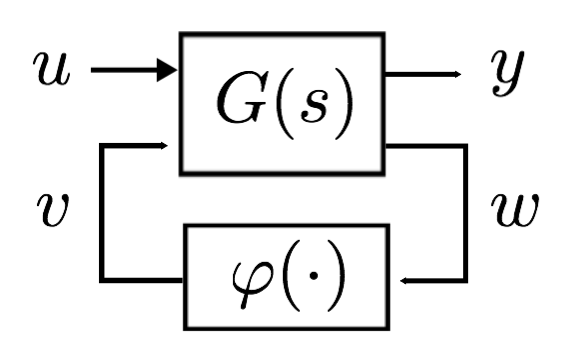
\includegraphics[width=1.5in]{picture/system_w_uncertainty.png}
	\caption{Lur\'e System representation of the swing equation with linearized dynamics in $G(s)$ and nonlinear components in $\varphi$.}
	\label{fig_system_w_uncertainty}
\end{figure}

\section{Input Output Stability Analysis with Sector Bound}

\begin{definition}
Given a multidimensional signal, $u(t)\in\mathbb{R}^n$, $\infty$-norm of the signal,  $|u|_\infty\in\mathbb{R}^n$, is defined here as
\begin{equation}
\big[|u|_\infty\big]_i=\sup_{t\geq0}|u_i(t)|
\end{equation}
where $\big[|u|_\infty\big]_i$ and $u_i$ are the $i$-th entry of $|u|_\infty$ and $u$ respectively.
\end{definition}

Note that this is different from standard $\mathcal{L}\infty$ norm of the multidimensional signal, $||u||_\infty=\max_i\big(\sup_{t\geq0}|u_i(t)|\big)$. Our definition allows optimization of each entry of the $\infty$-norm rather than $\mathcal{L}\infty$, which bounds the inputs and outputs uniformly. We exploit this flexibility and optimize for optimal maximum bound on the perturbation while guaranteeing the stability.

\begin{definition}
Suppose we are given a system, $G$, with input $u\in\mathbb{R}^m$ and output $y\in\mathbb{R}^{n}$. The $\infty$-gain matrix of the system, $\gamma\in\mathbb{R}^{n\times m}$, is defined as a matrix that satisfies
\begin{equation}
|y|_\infty\leq\gamma_G|u|_\infty.
\label{eqn_infty_gain}
\end{equation}
\end{definition}

For a linear system, we can compute the gain matrix using the following lemma.

\begin{lemma} (Bounded Input Bounded Output)
Given a linear system with $G$ as a $n$ by $m$ transfer function matrix, the $\infty$-gain matrix of the system is
\begin{equation}
\gamma_{ij}=||G_{ij}(t)||_1
\end{equation}
where $||G_{ij}(t)||_1=\int_{-\infty}^{\infty}|h_{ij}(\tau)|d\tau$ and $h$ is the impulse response of the transfer function, $G_{ij}$.

\label{lemma_BIBO}
\end{lemma}
\begin{proof}
For the $i$-th entry of output,
$$\begin{aligned}|y_i(t)|&=\bigg|\sum_j\int_{-\infty}^{\infty}h_{ij}(\tau)u_j(t-\tau)d\tau\bigg| \\
& \leq \sum_j\int_{-\infty}^{\infty}|h_{ij}(\tau)| |u_j(t-\tau)|d\tau \\
& \leq \sum_j\bar{u}_j\int_{-\infty}^{\infty}|h_{ij}(\tau)|d\tau \\
&=\sum_j||G_{ij}(t)||_1\bar{u}_j=\sum_j\gamma_{ij}\bar{u}_j.
\end{aligned}$$
\end{proof}

Let the $\infty$-gain matrix of $G$ in Equation \ref{eqn_G} is given by $\gamma_G\in\mathbb{R}^{(m+l)\times(n+l)}$

\begin{equation}
\gamma_G=\begin{bmatrix}
        \gamma_{y,u} & \gamma_{y,v} \\
        \gamma_{w,u} & \gamma_{w,v} \\
     \end{bmatrix}
\end{equation}
where $\gamma_{y,u}\in\mathbb{R}^{m\times n}$,  $\gamma_{y,v}\in\mathbb{R}^{m\times l}$,  $\gamma_{w,u}\in\mathbb{R}^{l\times n}$, and  $\gamma_{w,v}\in\mathbb{R}^{l\times l}$ are the respective components in the gain matrix. We can compute this gain using Lemma \ref{lemma_BIBO}, using numerical integration over the impulse response. Suppose we are also given the $\infty$-gain for the nonlinearities $\varphi$ is given by $\gamma_\varphi$. From the definition of $\infty$-gain in Equation  \ref{eqn_infty_gain}, the following inequalities holds:
\begin{equation}
|y|_\infty\leq\gamma_{y,u} |u|_\infty+\gamma_{y,v}|v|_\infty
\label{eqn_plant_y_gain}
\end{equation}
\begin{equation}
|w|_\infty\leq\gamma_{w,u} |u|_\infty+\gamma_{w,v}|v|_\infty
\label{eqn_plant_w_gain}
\end{equation}
\begin{equation}
|v|_\infty\leq\gamma_\varphi |w|_\infty.
\label{eqn_nonlinearity_gain}
\end{equation}

Before stating the result, we introduce a definition of monotone matrix and a lemma, which will be used for the theorem.

\begin{definition}
$A\in\mathbb{R}^{n\times n}$ is a monotone matrix if $Ax\geq 0$ implies $x\geq 0$ for all vector $x\in\mathbb{R}^{n}$.
\end{definition}

\begin{comment}
\begin{lemma}
$A$ is a monotone matrix, if and only if $A^{-1}\geq0$.
\label{lemma_mono_inv}
\end{lemma}
\begin{proof}
First we note that $A$ is nonsingular and invertable. We can see this since $Ax=0$ implies $x\geq0$ and $-x\geq0$, and hence $x=0$.
\newline($\Rightarrow$) Suppose A is monotone. Let $x$ be the $i$-th column of $A^{-1}$, then $Ax=\hat{e}_i\geq0$ where $\hat{e}_i$ is a unit vector. By the definition of monotonicity, $x$ is non-negative, and hence $A^{-1}$ is non-negative.
\newline($\Leftarrow$) Suppose $A^{-1}\geq 0$ and $Ax\geq 0$. Then $x=(A^{-1}A)x=A^{-1}(Ax)\geq 0$.
\end{proof}
\end{comment}

\begin{lemma}
The following statements are equivalent for the matrix, $I-\gamma_{w,v}\gamma_\varphi$, which has non-positive off-diagonal entries:
\begin{enumerate}[(i)]
\item $I-\gamma_{w,v}\gamma_\varphi$ is a monotone matrix,
\item $I-\gamma_{w,v}\gamma_\varphi\succ 0$,
\item There exists $\bar{w}\geq0$ such that $(I-\gamma_{w,v}\gamma_\varphi)\bar{w}>0$.
\end{enumerate}
\label{lemma_Zmatrix}
\end{lemma}

\begin{proof}
We skip the detailed proof for this lemma due to the space. Since $\gamma_{w,v}$ and $\gamma_\varphi$ have every entries non-negative, the off-diagonal elements of $I-\gamma_{w,v}\gamma_\varphi(\bar{w})$ are non-positive. This type of matrix is known as a $Z$-matrix. If $Z$-matrix satisfies the listed equivalent conditions, then the matrix is known as $M$-matrix. The list of papers linking to the proof can be found in \cite{plemmons77}. 
\end{proof}

Finally we are ready to state the small gain theorem for the $\infty$-norm we defined.
\begin{theorem}
\textit{(Small-Gain Theorem for $\infty$-norm)} The system with input $u$ and output $y$ is finite gain $\infty$-norm stable if  $\gamma_{w,v}\gamma_\varphi\prec I$.
\end{theorem}

\begin{proof}
By substituting Equation \ref{eqn_plant_w_gain} into Equation \ref{eqn_nonlinearity_gain}, we have
$$|w|_\infty\leq\gamma_{w,u} |u|_\infty+\gamma_{w,v}\gamma_\varphi |w|_\infty,$$
$$(I-\gamma_{w,v}\gamma_\varphi)|w|_\infty\leq\gamma_{w,u} |u|_\infty.$$
From the condition in the theorem, $I-\gamma_{w,v}\gamma_\varphi$ is positive definite, so it is a monotone matrix from Lemma \ref{lemma_Zmatrix} and is invertable. Then, we can write
$$(I-\gamma_{w,v}\gamma_\varphi)\big[(I-\gamma_{w,v}\gamma_\varphi)^{-1}\gamma_{w,u} |u|_\infty-|w|_\infty\big]\geq0,$$
which monotonicity of $I-\gamma_{w,v}\gamma_\varphi$ implies
$$(I-\gamma_{w,v}\gamma_\varphi)^{-1}\gamma_{w,u} |u|_\infty-|w|_\infty\geq0,$$
$$|w|_\infty\leq(I-\gamma_{w,v}\gamma_\varphi)^{-1}\gamma_{w,u} |u|_\infty.$$
Then the output can be bounded by
$$\begin{aligned} 
|y|_\infty&\leq\gamma_{y,u} |u|_\infty+\gamma_{y,v}|v|_\infty \\
&\leq\gamma_{y,u} |u|_\infty+\gamma_{y,v}\gamma_\varphi |w|_\infty \\ 
&\leq\big[\gamma_{y,u}+\gamma_{y,v}\gamma_\varphi (I-\gamma_{w,v}\gamma_\varphi)^{-1}\gamma_{w,u}\big] |u|_\infty.
\end{aligned}$$
Therefore, the output is bounded with finite gain.
\end{proof}

In general, the condition in small-gain theorem does not satisfy for our system. Our system is not BIBO stable for general input bound, however, there is a finite input bound such that our system is stable. For the nonlinear system, the system is not globally stable towards the desired equilibrium, and the state needs to stay close to the desired equilibrium. If this bound can be estimated, the gain for the nonlinear component, $\gamma_\varphi$, can be significantly reduced. Note that with this approach, $\gamma_\varphi(\bar{w})$ is a function of the estimated bound $\bar{w}$ on the input to the nonlinear component. Figure \ref{fig_sector_bound_cos} illustrates the idea of confining gain based on $\bar{w}$. In addition, we can modify the general small gain theorem result for our application.

\begin{figure}[!htbp]
	\centering
	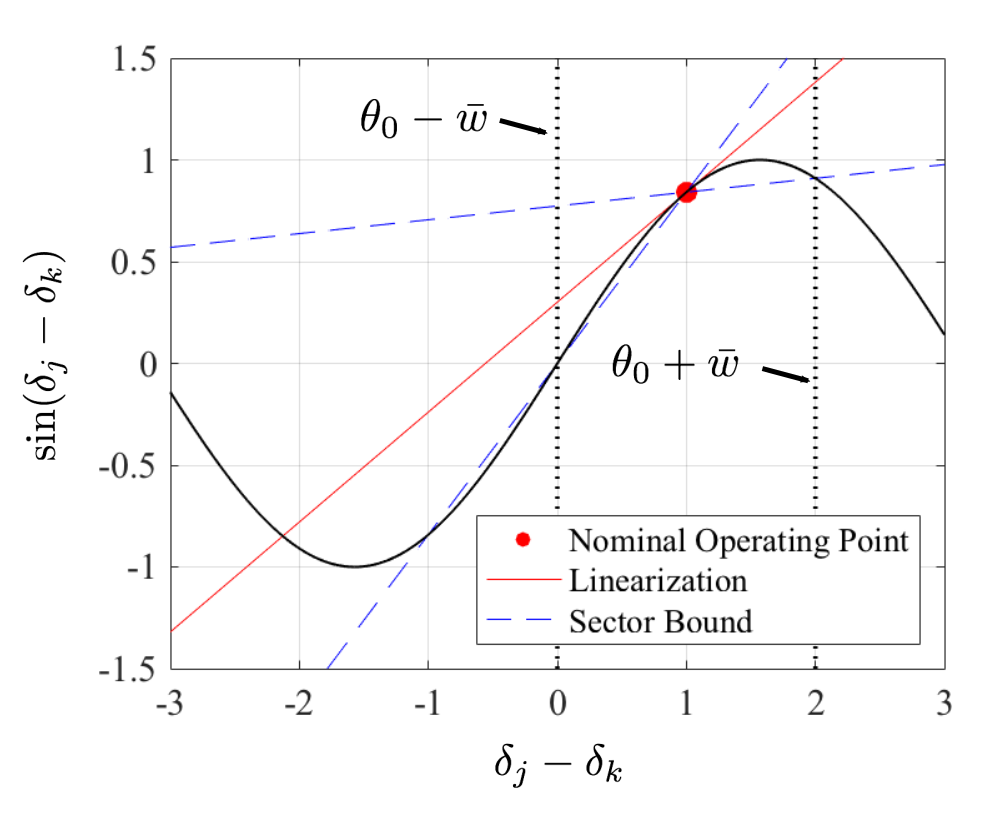
\includegraphics[width=3.2in]{picture/sector_bound_cos.png}
	\caption{Sector bound for sin function.}
	\label{fig_sector_bound_cos}
\end{figure}

In the next theorem, we actively employ the sector bound on the nonlinear term to compute the input bound that guarantees that the output is also stable. While the idea and the proof is simple, this result allows efficient ways to estimate to our problem. Before stating the theorem, we first write a lemma that will be used for the proof of our theorem.

\begin{theorem}
If $\gamma_{w,u}\bar{u}\leq(I-\gamma_{w,v}\gamma_\varphi(\bar{w}))\bar{w}$, then $|w|_\infty\leq\bar{w}$ for every $u$ such that $|u|_\infty\leq\bar{u}$.
\label{theorem_main}
\end{theorem}

\begin{proof}
Suppose there is a feasible solution $\bar{u}$, then $\gamma_{w,u}$ and $\bar{u}$ are matrix and vector with positive entries, and 
$(I-\gamma_{w,v}\gamma_\varphi(\bar{w}))\bar{w}\geq\gamma_{w,u}\bar{u}\geq0$ with $\bar{w}\geq0$. From Lemma \ref{lemma_Zmatrix}, $I-\gamma_{w,v}\gamma_\varphi(\bar{w})$ is a monotone matrix.
By substituting Equation \ref{eqn_plant_w_gain} into Equation \ref{eqn_nonlinearity_gain}, we have
$$|w|_\infty\leq\gamma_{w,u} |u|_\infty+\gamma_{w,v}\gamma_\varphi |w|_\infty.$$
We rearrange the equation and the substitution of conditions result in
$$\begin{aligned} 
0&\leq\gamma_{w,u} |u|_\infty-(I-\gamma_{w,v}\gamma_\varphi)|w|_\infty \\ 
&\leq\gamma_{w,u} \bar{u}-(I-\gamma_{w,v}\gamma_\varphi)|w|_\infty \\ 
&\leq(I-\gamma_{w,v}\gamma_\varphi(\bar{w}))\bar{w}-(I-\gamma_{w,v}\gamma_\varphi)|w|_\infty \\ 
&\leq(I-\gamma_{w,v}\gamma_\varphi(\bar{w}))(\bar{w}-|w|_\infty) \\ 
\end{aligned}$$
Since $I-\gamma_{w,v}\gamma_\varphi$ is a monotone matrix, $\bar{w}\geq|w|_\infty$.
\end{proof}

\begin{remark}
If $\bar{y}$ contains only the desired equilibrium, then any $\bar{u}$ that satisfies $\gamma_{w,u}\bar{u}\leq(I-\gamma_{w,v}\gamma_\varphi(\bar{w}))\bar{w}$ is the maximum input perturbation allowed to ensure the stability of the system. (Prove something like the solution will not converge to undesired equilibrium.)
\end{remark}

To find the maximum gain, the following optimization problem needs to be solved 
\begin{equation}
\begin{aligned}
& \underset{\bar{w}\geq 0,\ \bar{u}\geq 0}{\text{maximize}} & & c\bar{u} \\
& \text{subject to} & & \gamma_{w,u}\bar{u}\leq(I-\gamma_{w,v}\gamma_\varphi(\bar{w}))\bar{w}
\end{aligned}
\label{eqn_opt}
\end{equation}
The objective function $c\bar{u}$ is a linear function where the cost $c$ is determined to maximize perturbation which bus. For example, if a single generator or load bus is selected, then $c$ will be a unit vector with 1 at the index of selected bus. If Loads are uniformly perturbed, then $c$ will be 1 at the indices of the load buses.

We note that $\gamma_\varphi(\bar{w})$ is a monotonically increasing function with respect to $\bar{w}$. There are two competing effects which are
\begin{enumerate}
\item As $\bar{w}$ increases, $\gamma_\varphi$ increases. This increases the gain coming from the nonlinearities, so it reduces the certifiable range $\bar{u}$.
\item If $\bar{w}$ is too small, $\bar{u}$ has to be also bounded to ensure that the state does not reach $\bar{w}$.
\end{enumerate}
This observation is shown in the optimization problem in (\ref{eqn_opt}) where the objective is constrained by multiplication of monotonically increasing function $\bar{w}$ and monotonically decreasing function $(1-\gamma_{w,v}\gamma_\varphi(\bar{w}))$.

\section{Optimization Procedure with Sector Bound}
In this section, we derive explicit expression for the $\infty$-gain of nonlinear component and formulate optimization problem that can be solved efficiently.
\subsection{Adaptive Sector Bound}
The $\infty$-gain of $\varphi$ is defined as:
\begin{equation}
\gamma_\varphi(\bar{w})=\max_{0<w\leq\bar{w}}\bigg|\frac{\varphi(w)}{w}\bigg|
\end{equation}

The solution for the above equation is
\begin{equation}
\gamma_\varphi(\bar{w})=\text{diag}\big(\max\{|\bar{g}(\bar{w})|,|\underbar{$g$}(\bar{w})|\}\big)
\end{equation}
where $\bar{g}(\bar{w})$ and $\underbar{$g$}(\bar{w})$ are computed as follows:
\begin{equation}
\bar{g}(\bar{w})=\cos(\theta_0)-\frac{\sin(\theta_0)-\sin(\theta_0-\Delta \bar{w})}{\Delta \bar{w}}
\end{equation}
where $\Delta \bar{w}=\min\{\bar{w},\theta_0-\bar{\theta}_c\}$ and
$$\bar{\theta}_c=\min\bigg\{\theta_c \ \big| \ \frac{\sin(\theta_c)-\sin(\theta_0)}{\theta_c-\theta_0}=\cos(\theta_c), \ \theta_c>\theta_0 \bigg\}$$
and
\begin{equation}
\underbar{$g$}(\bar{w})=\cos(\theta_0)-\frac{\sin(\theta_0+\Delta \underbar{$w$})-\sin(\theta_0)}{\Delta \underbar{$w$}}
\end{equation}
where $\Delta \underbar{$w$}=\min\{\bar{w},\underbar{$\theta$}_c-\theta_0\}$ and
$$\underbar{$\theta$}_c=\max\bigg\{\theta_c \ \big| \ \frac{\sin(\theta_c)-\sin(\theta_0)}{\theta_c-\theta_0}=\cos(\theta_c), \ \theta_c<\theta_0 \bigg\}.$$

\begin{figure}[!htbp]
	\centering
	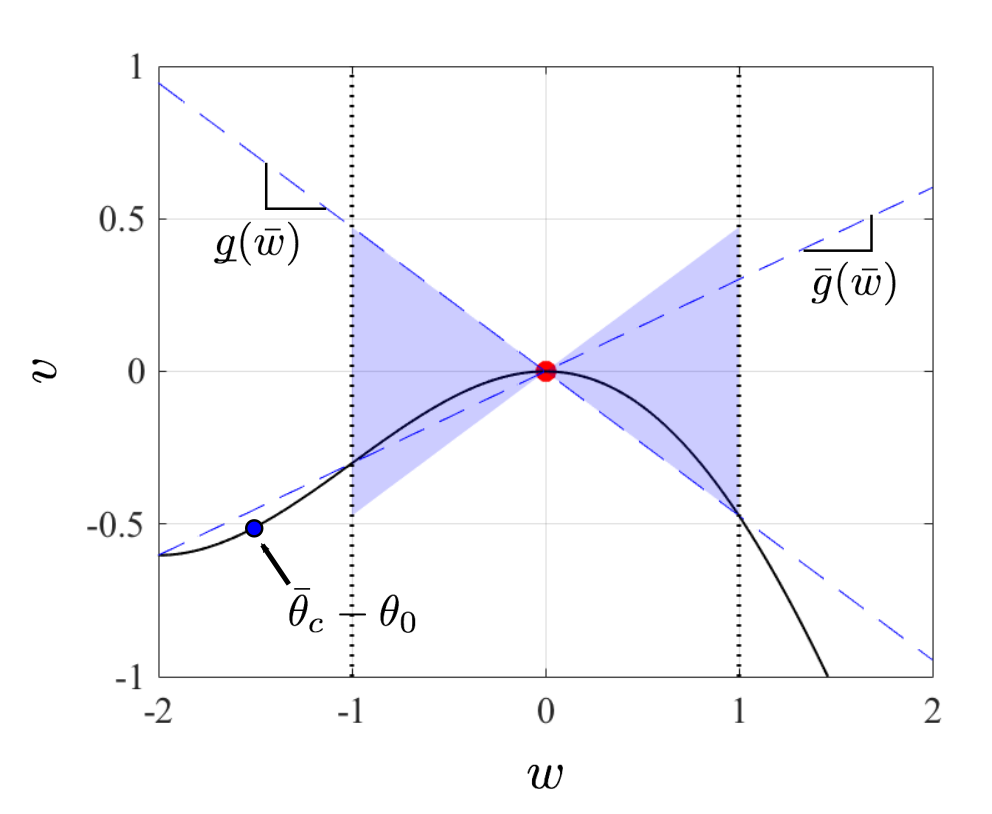
\includegraphics[width=3.2in]{picture/sector_bound_vw.png}
	\caption{Sector bound for sin function.}
	\label{fig_sector_bound_vw}
\end{figure}


This solution for the sector bound seems non-differentiable and complex, however if we bound the angle difference, then we can come up with an analytical expression that is much more simpler. We present this result in the following Corollary.

\begin{corollary}
Suppose $|\theta_0|=|E\delta_0|\leq\frac{\pi}{2}$ and $\bar{w}\leq\frac{\pi}{2}$. If $\theta_{i,0}=\delta_{k,0}-\delta_{j,0}\geq0$ then 
\begin{equation}
\gamma_{\varphi,ii}(\bar{w})=\cos(\theta_{i,0})-\frac{\sin(\theta_{i,0}+\bar{w}_i)-\sin(\theta_{i,0})}{\bar{w}_i}
\end{equation}
and if $\theta_{i,0}\leq0$ then 
\begin{equation}
\gamma_{\varphi,ii}(\bar{w})=\cos(\theta_{i,0})-\frac{\sin(\theta_{i,0})-\sin(\theta_{i,0}-\bar{w}_i)}{\bar{w}_i}
\end{equation}
\label{corollary_phigain}
\end{corollary}
\begin{proof}
Let us consider the case where $\theta_{i,0}\geq0$. 

and we will show $\underbar{$g$}_i(\bar{w})\geq|\bar{g}_i(\bar{w})|$. Given the conditions $|\theta_0|\leq\frac{\pi}{2}$ and $\bar{w}\leq\frac{\pi}{2}$, the following two inequalities hold:
$$\begin{aligned}
\underbar{$g$}_i(\bar{w})+\bar{g}_i(\bar{w}) &\geq 2\cos(\theta_{i,0})-\frac{\sin(\theta_{i,0}+\bar{w})-\sin(\theta_{i,0}-\bar{w})}{\bar{w}} \\
&=2\cos(\theta_{i,0})\bigg(1-\frac{\sin(\bar{w})}{\bar{w}}\bigg)\geq0,
\end{aligned}$$
$$\begin{aligned}
\underbar{$g$}_i(\bar{w})-\bar{g}_i(\bar{w}) &\geq \frac{2\sin(\theta_{i,0})-\sin(\theta_{i,0}+\bar{w})-\sin(\theta_{i,0}-\bar{w})}{\bar{w}} \\
&=\frac{2\sin(\theta_{i,0})}{\bar{w}}\big(1-\cos(\bar{w})\big)\geq0.
\end{aligned}$$
\end{proof}

Note if $\theta_{i,0}=0$, then both equations are the same since sin is an even function. Based on this expression, we can look at the original problem in (\ref{eqn_opt}).

\subsection{Computation of the Maximum Perturbation}
In this section, we discuss the estimation of maximum perturbation with provable stability. This is done by solving the optimization problem in (\ref{eqn_opt}). The problem is non-convex, we will show that the feasible region is convex.


\subsubsection{Estimation using Uniform Bound on $\bar{w}$}
An estimation of maximum perturbation can be computed if we let $\bar{w}$ be uniform for all angle differences. We note that if $\bar{w}$ is fixed, then the problem in (\ref{eqn_opt}) is a linear program. In addition, if the bound on the angle differences are uniform, then the decision variable is a scalar. The peak perturbation can be found by graphing $\bar{u}$ with respect to $\bar{w}$. However, the solution will be conservative since the angle difference bound is not optimized for each transmission line. In the next method, we will show that a local optimal point search method will efficiently find the solution.

\subsubsection{Interior Point Method}
Although the optimization problem in (\ref{eqn_opt}) is a non-convex problem, if we substitute the analytical expression for the non-linearity gain and bound the solution, then we can show that the feasible region of the constraint is actually convex.
To show this, first let $D=\text{diag}(\text{sign}(\theta_0))$ where $\theta_0=E\delta_0$, then we can rewrite the result from Corollary \ref{corollary_phigain} can be written as
\begin{equation}
\gamma_\varphi(\bar{w})=\text{diag}\bigg(\cos(\theta_0)+D\frac{\sin(\theta_0)-\sin(\theta_0-D\bar{w})}{\bar{w}}\bigg).
\end{equation}
Then, the substitution of the gain to the condition given in Theorem \ref{theorem_main} is as follows:
\begin{equation}
\begin{aligned}
\gamma_{w,u}\bar{u}&\leq(I+\gamma_{w,v}\text{diag}(\cos(\theta_0)))\bar{w} \\
& \hskip 3em -\gamma_{w,v}D\big(\sin(\theta_0)-\sin(\theta_0+D\bar{w})\big).
\end{aligned}
\end{equation}

Since sin is an even function,

\begin{equation}
\begin{aligned}
\gamma_{w,u}\bar{u}&\leq(I+\gamma_{w,v}\text{diag}(\cos(\theta_0)))\bar{w} \\
& \hskip 2em -\gamma_{w,v}D\sin(\theta_0)+\gamma_{w,v}\sin(|\theta_0|+\bar{w}).
\end{aligned}
\end{equation}

For this analytical expression we bounded $0\leq\bar{w}\leq \frac{\pi}{2}$ and $0\leq|\theta_0|\leq \frac{\pi}{2}$. Therefore, the input to the sinusoidal term is bounded by $0\leq|\theta_0|+\bar{w}\leq\pi$. Then, $\sin(|\theta_0|+\bar{w})$ is concave in that region multiplied by positive $\gamma_{w,v}$, and it has to be greater than some linear function. This constraint is convex over the feasible region. Now this optimization problem can be written as follow:

\begin{equation}
\begin{aligned}
& \underset{\bar{w},\ \bar{u}}{\text{maximize}} & & c\bar{u} \\
& \text{subject to} & & \gamma_{w,u}\bar{u}\leq(I+\gamma_{w,v}\text{diag}(\cos\theta_0))\bar{w} \\
& & & \hskip 2em -\gamma_{w,v}D\sin\theta_0+\gamma_{w,v}\sin(|\theta_0|+\bar{w}) \\
& & & 0\leq\bar{w}\leq \frac{\pi}{2}, \ 0\leq\bar{u}\leq \frac{\pi}{2}
\end{aligned}
\label{eqn_opt2}
\end{equation}
Since the feasible region of this optimization is convex, we expect interior point method to work well for this problem. We used IPOPT \cite{wachter06}. For the initial condition, we always know that $\bar{w}=0$ and $\bar{u}=0$ is a feasible solution.

\section{Case Studies}
\subsection{Single Machine Example}
\begin{equation}
m\ddot{\delta}+d\dot{\delta}+a\sin\delta=P
\end{equation}

Suppose the nominal operating condition is $\delta_0$ and $P_0$. By substituting $y=\delta-\delta_0$, $w=E(\delta-\delta_0)$, $u=P-P_0$, and $v=\sin(\delta)-\cos(\delta_0)y$,
\begin{equation}
m\ddot{y}+d\dot{y}+a(v+\cos(\delta_0)y)=u
\end{equation}

In frequency domain,
\begin{equation}
\begin{aligned}
Y&=\frac{1}{ms^2+ds+a\cos(\delta_0)}U-\frac{a}{ms^2+ds+a\cos(\delta_0)}V \\
&=G_uU+G_vV
\end{aligned}
\end{equation}

\begin{figure}[!htbp]
	\centering
	\includegraphics[width=3.2in]{picture/max_pert_2bus.png}
	\caption{Maximum perturbation allowed as a function of sector bound for 2 bus system.}
	\label{fig_max_perturbation_2bus}
\end{figure}


\begin{figure}[!htbp]
	\centering
	\includegraphics[width=3.2in]{picture/max_pert_39bus_loads.png}
	\caption{Result for 39 bus system with uniformly bounded loads by $\Delta P_{max}$. The upper bound was obtained by letting $u =\Delta P_{max}$ for all time.}
	\label{fig_max_perturbation_2bus}
\end{figure}


\begin{figure}[!htbp]
	\centering
	\includegraphics[width=3.2in]{picture/max_pert_39bus_singlebus.png}
	\caption{Result for 39 bus system with single load bounded by $\Delta P_{max}$. The upper bound was obtained by letting $u =\Delta P_{max}$ for all time.}
	\label{fig_max_perturbation_2bus}
\end{figure}

To Do List:
\begin{enumerate}
\item Add details to Lemma III.1
\item Prove the solution will not converge to any undesired solution
\item Put results
\end{enumerate}

Future Extensions
\begin{enumerate}
\item Adaptive linearization/gain
\item identify worst case $u$, link to cyber attack
\item Find ROA using impulse as initial condition
\item Can we bound both energy and maximum? Application for fault analysis
\end{enumerate}

%\appendices

\ifCLASSOPTIONcaptionsoff
\newpage
\fi

\bibliographystyle{IEEEtran}
\bibliography{references}
\nocite{*} 

\end{document}







